\begin{frame}{Acceleration with Tensor Cores}
	

		\begin{columns}
			\column{0.5\textwidth}
			\hfill Recent NVIDIA GPUs
			
			\hfill (Volta Architecture)
			\column{0.5\textwidth}
			\begin{itemize}
				\item Refined scheduler
				\item New memory scheme
				\item Tensor Cores
			\end{itemize}
		\end{columns} 


	\begin{center}
		\begin{minipage}{0.88\textwidth}
			\begin{columns}
				\column{0.6\linewidth}
				Tensor Cores:
				\begin{itemize}
					\item[WHAT] Matrix-matrix multiplication
					\item[HOW] Mixed precision (precision loss)
					\item[WHY] Originally, deep learning
				\end{itemize}
				\column{0.5\linewidth}
				\begin{figure}
					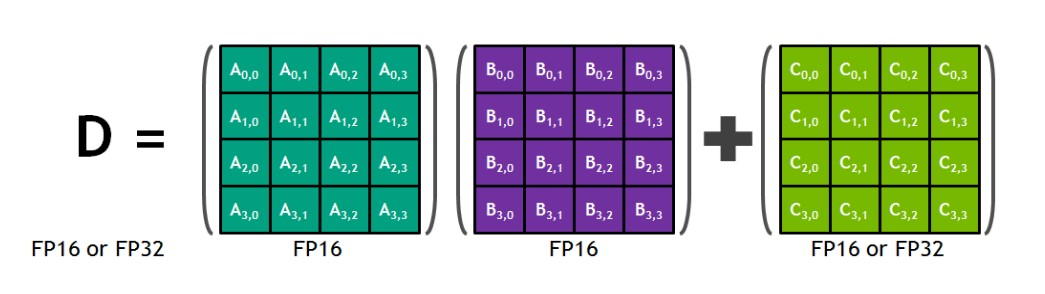
\includegraphics[width=\textwidth]{tensor_core_op}
					\caption{Operation done by a Tensor Core}
				\end{figure}
			\end{columns}
		\end{minipage}
	
	\begin{minipage}{0.70\textwidth}
	Could be used to calculate:
	
	\begin{itemize}
		\item B-Splines (quantify smoothness)
		\item Entropy (quantify similarity)
	\end{itemize}
	
	And other various modern optimizations
	\end{minipage}
	\end{center}

		
\end{frame}